\documentclass[a4paper,12pt,reqno]{article}

\usepackage{styledoc19}


\begin{document} % конец преамбулы, начало документа

    \year{2022}
    \docNumber{RU.17701729.04.01-01 34 01-1}
    \docFormat{Руководство оператора}
    \student{БПИ 183}{А. А. Глушко}

    \project{Автоматическая генерация и проверка учебных заданий на основе онтологии предметной области для систем персонализированного адаптивного обучения}


    \supervisor{Доцент Факультет компьютерных \vfill наук анализа данных и \vfill искусственного интеллекта  \vfill }
    {А. А. Незнанов}

    \firstPage
    \newpage
    \secondPage
    \newpage
    \thirdPage
    \newpage


    \section{Назначение программы}

    \subsection{Функциональное назначение}
    Разрабатываемое решение предоставляет возможность генерировать контрольно-измерительные материалы с имитационной моделью и эталонным решением на основе онтологии учебного процесса и онтологии предметной области. Для демонстрации генератора дополнительно разрабатывается расчетный модуль, который позволяет пользователю запросить контрольно-измерительные материалы, решить предложенные задания и получить оценку. Также поддерживается назначения учебного задания для пользователя учителем при помощи интеграции с LMS.

    \subsection{Эксплуатационное назначение}
    Подсистема ГПРЗ (генерация и проверка расчетных заданий) должна использоваться в программных средствах учебного назначения (ПСУН), поддерживающих персонализированный адаптивный учебный процесс. Конечными пользователями таких ПСУН являются школьники и студенты, учебным планом которых предусмотрено обучение решению расчетных задач.

    \subsection{Область применения}
    В последнее время заметно активное развитие адаптивных программных систем. Во многом это связано с опровержением гипотезы о среднем человеке \cite{introduction:average_person}, заключающейся в том, что, ориентируя систему на среднего пользователя, она будет удобна большинству. На практике оказалось, что современные программные системы имеют огромное количество критериев удобства и, подбирая их для комфорта среднего человека, система оказывается неудобна никому \cite{introduction:average_person_UX}. Выходом стало развитие адаптивных программных систем, которые способны подстраиваться под пользователя.

    Особенно актуальными такие системы оказались для образования, так как каждый ученик уникален, и невозможно придумать универсальный алгоритм обучения, который будет удобен всем. Это привело к развитию систем персонализированного адаптивного обучения или Personalized Adaptive Learning Systems (PALS). Это достаточно широкий класс систем. В нашей работе мы будем рассматривать пересечение PALS систем и интерактивных тьютеринговых систем (Intelligent tutoring system, ITS). Такие системы базируются на идеи Льва Выготского (Lev Vygotsky) о зоне ближайшего развития \cite{introduction:ZPD_1} \cite{introduction:ZPD_2} (Zone of proximal Development). Лев Выготский определил зону ближайшего развития как область знаний, которую учащийся может освоить при поддержке более опытного (More Knowledgeable Other). При этом важно отметить, что в роли более опытного может выступать учитель, одноклассник или даже компьютерная система. Важно, чтобы в процессе изучения знаний из области ближайшего развития ученику была оказанная поддержка, которая в педагогике называется скаффолдингом \cite{scaffolding:Belland} \cite{scaffolding:cognitive}. Существует множество различных методов скаффолдинга, и это широко обсуждаемая тема среди преподавателей \cite{scaffolding:strategies_1} \cite{scaffolding:strategies_2}.

    Для того, чтобы система могла выступать в качестве <<More Knowledgeable Other>> и помочь обучаемому осваивать новые знания и навыки, она должна обладать возможностью предоставить пользователю релевантное задание, на основе взаимодействия пользователя с заданием определить его лакуны в знаниях (Knowledge gaps) и применить подходящий метод скаффолдинга для устранения данной лакуны.
    Существует множество систем, которые реализуют данный функционал. Наиболее известным примером является ALEKS \cite{competitors:ALEKS}. Общей проблемой существующих на рыке систем является использования заранее заготовленного банка контрольно-измерительных материалов. Это приводит к необходимости постоянного обновления и дополнения банка, а также к сложностям при валидации и актуализации заданий \cite{introduction:KnowledgeLearningSpaces}\cite{introduction:KnowledgeSpaces}.
    Система, описанная в данном техническом задании, призвана попытаться решить данную проблему с помощью онтологически-контролируемого генератора заданий, учитывающего потребности современных PALS систем, особенно в области поддержки методов скаффолдинга.

    \subsection{Состав выполняемых функций}

    \subsubsection{Генератор контрольно-измерительных материалов}
    Генератор контрольно-измерительных материалов выполняет следующие функции:
    \begin{enumerate}
        \item генерирует аналитическую модель задания;
        \item генерирует задание с имитационной моделью;
        \item создает эталонное решение сгенерированного задания;
        \item вычисляет ответа на вопрос задания на основе эталонного решения;
        \item генерирует текст задания с помощью шаблона и имитационной модели.
    \end{enumerate}

    \subsection{Расчетная подсистема}
    Расчетная подсистема выполняет следующие функции:
    \begin{enumerate}
        \item предоставление возможности аунтификации в системе с возможностью смены пароля и редактирования профиля;
        \item отображение списка контрольно-измерительных мероприятий пользователя со статусом выполнения;
        \item предоставление возможности пользователю создать контрольно-измерительных мероприятий для самостоятельной практики;
        \item отображение списка заданий в рамках контрольно-измерительного мероприятия со статусом выполнения задания;
        \item предоставление интерфейса для решения задания с возможностью получения результатов.
    \end{enumerate}

    \newpage


    \section{Условия выполнения программы}

    \subsection{Минимальный состав аппаратурных средств}
    Для надежной и бесперебойной работы программы требуется следующий состав аппаратурных средств:
    \begin{enumerate}
        \item Компьютер, оснащенный процессором Intel Core i5 с тактовой частотой 2,3 ГГц;
        \item 16 Гб ОЗУ;
        \item Жесткий диск с объемом свободной памяти более чем 50 ГБ;
        \item Клавиатура и мышь;
        \item Доступ в интернет.
    \end{enumerate}

    \subsection{Минимальный состав программных средств}
    Для надежной и бесперебойной работы программы требуется следующий состав программных средств:
    \begin{enumerate}
        \item macOS 10.15.4 или Windows 10
        \item Google Chrome;
        \item Docker.
    \end{enumerate}

    \subsection{Требования к пользователю}
    Пользователь должен быть ознакомлен с терминологией, представленной в Приложении \ref{additionterms}. Также пользователь должен быть знаком на базовом уровне с аппаратурными средствами.

    \newpage


    \section{Загрузка и запуск программы}
    Для запуска разработанных сервисов скачайте репозиторий по адресу \url{https://github.com/Badcat330/EdMachine}.

    \subsection{Запуск генератор контрольно-измерительных материалов}
    Для запуска генератора необходимо перейти в директорию генератора и с помощью Docker файла собрать образ генератора. Затем необходимо запустить контейнер из собранного образа, указав следующие переменные среды:
    \begin{itemize}
        \item AUTHORSHIP: название генератора;
        \item VERSION: версия генератора;
        \item ONTOLOGY\_HOST: адрес подсистемы управления онтологиями.
    \end{itemize}

    \subsection{Запуск серверной части расчетная подсистема}
    Для запуска серверной части расчетной подсистемы необходимо перейти в ее директорию и с помощью Docker файла собрать образ. Затем необходимо запустить контейнер из собранного образа, указав следующие переменные среды:
    \begin{itemize}
        \item BANK\_HOST: адрес развернутого банка контрольно-измерительных материалов;
        \item EMAIL\_SENDER: адрес учетной записи, с которой будут отправляться уведомления;
        \item EMAIL\_PASSWORD: пароль от учетной записи;
        \item FRONT\_HOST: адрес развернутой клиентской части расчетной подсистемы;
        \item MATERIALS\_HOST: адрес подсистемы управления учебными материалами;
        \item ONTOLOGY\_HOST: адрес подсистемы управления онтологиями;
        \item SQLALCHEMY\_DATABASE\_URI: ссылка на подключение к базе данных.
    \end{itemize}

    \subsection{Запуск клиентской части расчетная подсистема}
    Для запуска клиентской части расчетной подсистемы необходимо перейти в ее директорию и с помощью Docker файла собрать образ. Затем необходимо запустить контейнер из собранного образа, указав следующие переменные среды:
    \begin{itemize}
        \item BACKEND\_HOST: адрес развернутой серверной части расчетной подсистемы.
    \end{itemize}


    \section{Выполнение программы}

    \subsection{Работа с генератором контрольно-измерительных материалов}
    Для описания API генератора использовался Swagger (см. рисунок \ref{pic:apig}). API генератора состоит из следующих запросов:
    \begin{enumerate}
        \item GET /health/check: используется для получения статуса сервиса;
        \item POST /generator/create: используется для генерации нового контрольно-измерительного материала на основе шаблона.
    \end{enumerate}
    Более подробно с интерфейсом генератора контрольно-измерительных материалов и примерами запросов Вы можете ознакомиться по ссылке \url{https://app.swaggerhub.com/apis/Badcat330/task-generator/}.

    \begin{figure}[H]
        \centering
        \includegraphics[width=\linewidth]{img/APIG.png}
        \caption{API генератора контрольно-измерительных материалов в Swagger}
        \label{pic:apig}
    \end{figure}

    \subsection{Работа с расчтеной подсистемой}

    \subsubsection{Главная страница}

    На данной странице представлено приветственное сообщение и кнопка для перехода к списку контрольно-измерительных мероприятий (см. рисунок \ref{pic:home}). В случае, если пользователь еще не аунтифицировался в системе, его автоматически переведет на страницу аунтификации.

    \begin{figure}[H]
        \centering
        \includegraphics[width=\linewidth]{img/home.png}
        \caption{Интерфейс домашней страницы расчетной подсистемы}
        \label{pic:home}
    \end{figure}

    \subsubsection{Страница аунтификации}
    На данной странице пользователю предлагается ввести логин и пароль для входа в систему (см. рисунок \ref{pic:login}). При вводе данных пароль будет захэширован криптографическим хэшем SHA256 и отправлен на проверку в серверную часть расчетной подсистемы. Также с помощью гиперссылок, расположенных под кнопкой Log in Вы можете перейти на страницу регистрации или на страницу отправки заявки на сброса пароля.

    \begin{figure}[H]
        \centering
        \includegraphics[width=\linewidth]{img/login.png}
        \caption{Интерфейс страницы аунтификации пользователя в расчетной подсистеме}
        \label{pic:login}
    \end{figure}

    \subsubsection{Страница регистрации}
    На данной странице вы можете заполнить форму для регистрации в системе, а также перейти по гиперссылкам к странице аунтификаии или странице отправки заявки на сброс пароля (см. рисунок \ref{pic:signup}).

    \begin{figure}[H]
        \centering
        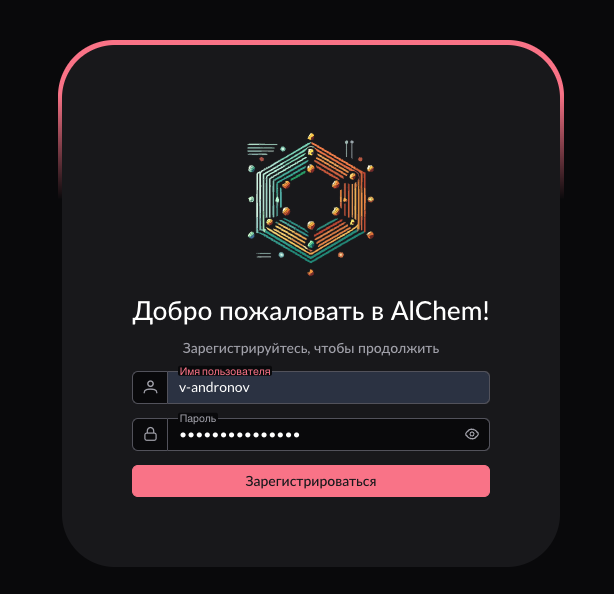
\includegraphics[width=\linewidth]{img/signup.png}
        \caption{Интерфейс страницы регистрации пользователя в расчетной подсистеме}
        \label{pic:signup}
    \end{figure}

    \subsubsection{Страница отправки заявки для сброса пароля}
    На данной странице Вы можете указать свой email, на который придет письмо с ссылкой для сброса пароля. (см. рисунок \ref{pic:find})

    \begin{figure}[H]
        \centering
        \includegraphics[width=\linewidth]{img/find.png}
        \caption{Интерфейс страницы запроса сброса пароля пользователя в расчетной подсистеме}
        \label{pic:find}
    \end{figure}

    \subsubsection{Страница сброса пароля}
    На данную страницу возможно попасть при переходе по ссылке для сброса пароля. Здесь Вы можете указать новый пароль, который будет присвоен вашей учетной записи (см. рисунок \ref{pic:reset}).

    \begin{figure}[H]
        \centering
        \includegraphics[width=\linewidth]{img/reset.png}
        \caption{Интерфейс страницы запроса сброса пароля пользователя в расчетной подсистеме}
        \label{pic:reset}
    \end{figure}

    \subsubsection{Персональная страница пользователя}

    На данной странице вы можете просмотреть данные о своей учетной записи, а также изменить их (см. рисунок \ref{pic:me}). При нажатии на кнопку edit поля с данными становятся активными для редактирования информации, и появляется возможность изменения данных и их сохранения в системе (см. рисунок \ref{pic:me_edit}). В случае, когда Вы не хотите менять данные, нажмите на кнопку cancel. Также Вы можете выйти из учетной записи, нажав кнопку sign out.

    \begin{figure}[H]
        \centering
        \includegraphics[width=\linewidth]{img/me.png}
        \caption{Интерфейс персональной страницы пользователя в расчетной подсистеме}
        \label{pic:me}
    \end{figure}

    \begin{figure}[H]
        \centering
        \includegraphics[width=\linewidth]{img/me_edit.png}
        \caption{Интерфейс персональной страницы пользователя в режиме редактирования в расчетной подсистеме}
        \label{pic:me_edit}
    \end{figure}

    \subsubsection{Список контрольно-измерительных мероприятий}
    На данной странице представлен список контрольно-измерительных мероприятий пользователя (см. рисунок \ref{pic:assessment_list}). В списке указано название контрольно-измерительного мероприятия и дата начала и окончания, для персональных мероприятий дата отсутствует. Справа также указывается статус выполнения. В случае выполнения всего мероприятия появляется иконка, символизирующая успешное прохождение. Также пользователь может перейти на страницу создания персонального мероприятия по нажатию кнопки Make personal assessment.

    \begin{figure}[H]
        \centering
        \includegraphics[width=\linewidth]{img/assessment_list.png}
        \caption{Интерфейс списка контрольно-измерительных мероприятий для пользователя в расчетной подсистеме}
        \label{pic:assessment_list}
    \end{figure}

    \subsubsection{Страница создания персонального контрольно-измерительного мероприятия}
    На данной странице представлена форма, заполнив которую Вы можете отправить заявку на создание для Вас контрольно-измерительного мероприятия (см. рисунок \ref{pic:personal_assessment}). В данной форме необходимо указать название мероприятия, тип заданий, количество заданий и флаг обязательной генерации. В случае, когда флаг отсутствует, задания будут генерироваться только при отсутствии подходящих в банке.

    \begin{figure}[H]
        \centering
        \includegraphics[width=\linewidth]{img/personal_assessment.png}
        \caption{Интерфейс создания персонального контрольно-измерительного мероприятия в расчетной подсистеме}
        \label{pic:personal_assessment}
    \end{figure}

    \subsubsection{Список заданий контрольно-измерительного мероприятия}

    На данной странице представлен список заданий контрольно-измерительного мероприятия и статус их выполнения (см. рисунок \ref{pic:task_list}). Также для каждого задания указан его формат и тип. При нажатии на задание Вы перейдете к его выполнению.

    \begin{figure}[H]
        \centering
        \includegraphics[width=\linewidth]{img/task_list.png}
        \caption{Интерфейс списка зданий контрольно-измерительного мероприятия в расчетной подсистеме}
        \label{pic:task_list}
    \end{figure}

    \subsubsection{Страница выполнения задания}
    На данной странице Вы можете ознакомиться с условием задания и ввести ответ (см. рисунок \ref{pic:solve_task}). По нажатию кнопки Submit задание отправится на проверку. В случае некорректного выполнения задания Вам будет предложено ознакомиться с учебными материалами, собранными на основе модели задания (см. рисунок \ref{pic:solve_definitions}).

    \begin{figure}[H]
        \centering
        \includegraphics[width=\linewidth]{img/solve_task.png}
        \caption{Интерфейс решения задания в расчетной подсистеме}
        \label{pic:solve_task}
    \end{figure}

    \begin{figure}[H]
        \centering
        \includegraphics[width=\linewidth]{img/solve_definitions.png}
        \caption{Пример ответа системы на некорректно решенное задание в расчетной подсистеме}
        \label{pic:solve_definitions}
    \end{figure}

    \newpage


    \section{Сообщения оператору}

    \subsection{Некорректная почта или пароль}
    В данном сообщении система сообщает о некорректности пары почта, пароль (см. рисунок \ref{pic:error_login}).

    \begin{figure}[H]
        \centering
        \includegraphics[width=\linewidth]{img/error_login.png}
        \caption{Сообщение о некорректной паре адреса почты и пароля}
        \label{pic:error_login}
    \end{figure}

    \subsection{Занятый почтовый адрес}
    Данное сообщение возникает при регистрации, если указанный почтовый адрес уже используется пользователем (см. рисунок \ref{pic:error_email}). В случае, если пользователь забыл свой пароль, он может пройти процедуру сбрасывания пароля.

    \begin{figure}[H]
        \centering
        \includegraphics[width=\linewidth]{img/error_email.png}
        \caption{Сообщение при попытке регистрации с уже занятым почтовым адресом}
        \label{pic:error_email}
    \end{figure}

    \subsection{Несовпадение пары паролей}
    Данное сообщение возникает в случае несовпадения повторного ввода пароля (см. рисунок \ref{pic:error_password}).

    \begin{figure}[H]
        \centering
        \includegraphics[width=\linewidth]{img/error_password.png}
        \caption{Пример сообщения при несовпадении повторного ввода пароля}
        \label{pic:error_password}
    \end{figure}

    \subsection{Незаполненное обязательное поле формы}
    Данное сообщение возникает в случае попытки отправки формы без заполнения одного из обязательных полей (см. рисунок \ref{pic:error_field}).

    \begin{figure}[H]
        \centering
        \includegraphics[width=\linewidth]{img/error_field.png}
        \caption{Пример сообщения при отправке формы без обязательного поля}
        \label{pic:error_field}
    \end{figure}

    \newpage
    \printbibliography[title=Список источников, heading=bibintoc]

    \newpage
    \addition{Используемые понятия и определения}{additionterms}
    \phantomsection
\addcontentsline{toc}{section}{Основные определения, термины и сокращения}

\begin{description}[style=unboxed,leftmargin=0cm]

    \item[\textbf{Валидность}] -- степень соответствия полученных данных реальности.

    \item[\textbf{Вычислительный эксперимент}] -- метод исследования, при котором математические модели и компьютерные расчёты используются для анализа сложных систем и прогнозирования их поведения.

    \item[\textbf{Домен (предметная область)}] -- область знаний, к которой относится конкретное программное обеспечение.

    \item[\textbf{Интероперабельность}] -- возможность обмена и понимания данных между разными системами на основе их смыслового значения.

    \item[\textbf{Клиент-серверная архитектура}] -- принцип проектирования ПО, согласно которому клиент запрашивает данные у сервера, который их обрабатывает и отправляет обратно.

    \item[\textbf{Лабораторный эксперимент}] -- метод научного исследования, проводимый в контролируемых условиях лаборатории для проверки гипотез, изучения свойств объектов или выявления закономерностей.

    \item[\textbf{Онтология}] -- формализованное представление знаний в определённой предметной области, включающее определения понятий, их свойства и взаимосвязи между ними. Используется в искусственном интеллекте, базах знаний и прочих областях.

    \item[\textbf{Слоистая архитектура}] -- принцип проектирования ПО, согласно которому система разделена на слои, каждый из которых выполняет свою роль.

    \item[\textbf{СУБД (Система управления базами данных)}] -- программное обеспечение для создания, управления и работы с базами данных.

    \item[\textbf{API (Application Programming Interface)}] -- интерфейс программирования приложений, набор правил и инструментов для взаимодействия между программными компонентами.

    \item[\textbf{ELN (Electronic Laboratory Notebook)}] -- электронный лабораторный журнал, который используется для ведения, хранения и управления научными записями, заменяя традиционные бумажные записи.

    \item[\textbf{JWT (JSON Web Token)}] -- компактный и безопасный способ передачи информации между сторонами в виде JSON-объекта, часто используется для аутентификации.

    \item[\textbf{ORM (Object-Relational Mapping)}] -- технология, позволяющая работать с базами данных с использованием объектно-ориентированных подходов вместо SQL-запросов.

    \item[\textbf{SPA (Single Page Application)}] -- веб-приложение, которое загружается один раз и обновляет контент без полной перезагрузки страницы, улучшая пользовательский опыт.

\end{description}

    \newpage
    \listRegistration

\end{document}